\documentclass[xcolor=dvipsnames,table]{beamer}

\usepackage{latexsym}
\usepackage[utf8]{inputenc}
\usepackage[brazil]{babel}
\usepackage{amssymb}
\usepackage{amsmath}
\usepackage{stmaryrd}
\usepackage{fancybox}
\usepackage{datetime}
\usepackage[T1]{fontenc}
\usepackage{graphicx}
\usepackage{graphics}
\usepackage{url}
\usepackage{algorithmic}
\usepackage{algorithm}
\usepackage{acronym}
\usepackage{array}

\newtheorem{definicao}{Definio}
\newcommand{\tab}{\hspace*{2em}}

\mode<presentation>
{
  \definecolor{colortexto}{RGB}{0,0,0}
 
  \setbeamertemplate{background canvas}[vertical shading][ bottom=white!10,top=white!10]
  \setbeamercolor{normal text}{fg=colortexto} 

  \usetheme{Warsaw}
}

\title{Grafo Conexo e Componente} 

\author{
  Esdras Lins Bispo Jr. \\ \url{bispojr@ufg.br}
  } 
 \institute{
  Teoria de Grafos \\Bacharelado em Ciência da Computação}
\date{\textbf{24 de maio de 2016} }

\logo{
\includegraphics[width=1cm]{images/ufgJataiLogo.png}}

\begin{document}

	\begin{frame}
		\titlepage
	\end{frame}

	\AtBeginSection{
		\begin{frame}{Sumário}%[allowframebreaks]{Sumário}
    		\tableofcontents[currentsection]
    		%\tableofcontents[currentsection, hideothersubsections]
		\end{frame}
	}

	\begin{frame}{Plano de Aula}
		\tableofcontents
		%\tableofcontents[hideallsubsections]
	\end{frame}
	
	\section{Pensamento}
	\begin{frame}{Pensamento}
  		\begin{center}
    		
\includegraphics[width=7cm]{images/pensamento.png}
  		\end{center}
	\end{frame}
	
	\begin{frame}{Pensamento}
		\begin{columns}
			\column{.4\textwidth}  		
		  		\begin{center}
		    		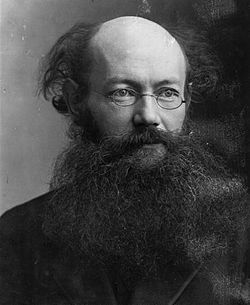
\includegraphics[height=.6\textheight]{images/kropotkin.jpg}
		  		\end{center}
			\column{.6\textwidth}  		
				\begin{block}{Frase}
					\begin{center}
						{\large Nenhuma revolução social pode triunfar se não for precedida de uma revolução nas mentes e corações do povo.}
					\end{center}
				\end{block}		  		
		  		\begin{block}{Quem?}
		  			\begin{center}
						{\bf Piotr Kropotkin (1842-1921)} \\Geógrafo e escritor russo.
					\end{center}
				\end{block}
		\end{columns}
	\end{frame}
	
	\begin{frame}{Bônus (0,5 pt)}
		\begin{block}{Desafio}
			\begin{itemize}
				\item Quanto valem os parâmetros $m$, $\delta$, e $\Delta$ de \\uma roda com $n$ vértices? (ver E 1.76); 
                \item Candidaturas até dia 24 de maio, 13h30; 
                \item Apresentação e resposta por escrito $\rightarrow$ \\(07 de junho, 15h30); 
                \item 20 minutos de apresentação.
			\end{itemize}
		\end{block} 	
	\end{frame}
    
    \section{Revisão}
	\subsection{Caminhos e Circuitos}
	\begin{frame}[shrink]{Caminhos e Circuitos}
		\begin{block}{Caminho}
			Um grafo $G$ é um {\bf caminho} se $V_G$ admite uma permutação $(v_1, v_2, \ldots , v_n)$ tal que
			\begin{center}
				$E_G = \{ v_i v_{i +1} : 1 \leq i < n \}$
			\end{center} 
			\begin{itemize}
				\item os vértices $v_1$ e $v_n$ são os {\bf extremos} do caminho; 
				\item os demais vértices são {\bf internos}; 
				\item diremos que esse caminho {\bf liga} $v_1$ a $v_n$.
			\end{itemize}
		\end{block} 
		\begin{block}{Notação}
			Podemos denotar um caminho pela sequência representada pelos seus vértices: 
			\begin{center}
				$v_1 v_2 \ldots v_n$		
			\end{center}
		\end{block}
	\end{frame}
	
	\begin{frame}[shrink]{Caminhos e Circuitos}
		\begin{block}{Circuito}
			Um grafo $G$ é um {\bf circuito} se $V_G$ tem 3 ou mais elementos e admite uma permutação $(v_1, v_2, \ldots , v_n)$ tal que
			\begin{center}
				$E_G = \{ v_i v_{i +1} : 1 \leq i < n \} \cup \{ v_1 v_n \}$
			\end{center} 
		\end{block} 
		\begin{block}{Notação}
			\begin{itemize}
				\item Podemos denotar um circuito simplesmente por: 
					\begin{center}
						$v_1 v_2 \ldots v_n v_1$		
					\end{center}
				\item O {\bf comprimento} de um caminho ou circuito $G$ é o número $m(G)$; 
				\item Um {\bf triângulo, quadrado, pentágono {e} hexágono} é o mesmo que um circuito de comprimento 3, 4, 5 e 6 respectivamente.
			\end{itemize}
		\end{block}
	\end{frame}
	
	\subsection{Subgrafos}
	\begin{frame}{Subgrafos}
		\begin{block}{Definição}
			Um {\bf subgrafo} de um grafo $G$ é qualquer grafo $H$ tal que $V_H \subseteq V_G$ e $E_H \subseteq E_G$.
		\end{block} 
		\begin{block}{Notações e Nomenclaturas}
			\begin{itemize}
				\item É conveniente escrever ``$H \subseteq G$'' para dizer que $H$ é subgrafo de $G$; 
				\item Um subgrafo $H$ de $G$ é {\bf gerador} ({\it abrangente}, para alguns) se $V_H = V_G$; 
				\item Um subgrafo $H$ de $G$ é {\bf próprio} se $V_H \not= V_G$ ou $E_H \not= E_G$ (notação: $H \subset G$).
			\end{itemize}
		\end{block}
	\end{frame}
	
	\begin{frame}{Subgrafos}
		\begin{block}{Subgrafo induzido - $G[X]$}
			O subgrafo de $G$ {\bf induzido} por um subconjunto $X$ de $V_G$ é o grafo $(X, F)$ em que $F$ é o conjunto $E_G \cap X^{(2)}$. \\Esse subgrafo é denotado por $G[X]$.
		\end{block} 
		\begin{block}{$G - X$}
			Para qualquer subconjunto $X$ de $V_G$, \\denotaremos por $G - X$ o subgrafo $G[V_G \setminus X]$.
		\end{block} 
		\begin{block}{$G - v$}
			Uma abreviação para $G - \{ v \}$.
		\end{block}
	\end{frame}
	
	\begin{frame}{Subgrafos}
		\begin{block}{$G - a$}
			Uma abreviação para o grafo $(V_G, E_G \setminus \{ a \})$.
		\end{block} 
		\begin{block}{$G - A$}
			Se $A$ é um subconjunto de $E_G$, então $G - A$ é uma abreviação para o grafo $(V_G, E_G \setminus A)$.
		\end{block} 
		\begin{block}{Corolário}
			$G - A$ é um grafo gerador de $G$.
		\end{block}
	\end{frame}
	
	\section{Grafos Conexos e Componentes}
	\begin{frame}{Grafos Conexos}
		\begin{block}{Definição}
			Um grafo é {\bf conexo} se, para qualquer par $\{v,w\}$ de seus vértices, existe um caminho com extremos $v$ e $w$.
		\end{block} \pause
		\begin{block}{Subgrafo conexo maximal}
			Um subgrafo conexo $H$ de um grafo $G$ é maximal se $H$ não é subgrafo próprio de algum subgrafo conexo de $G$.
		\end{block} \pause
		\begin{block}{Componente}
			Um {\bf componente} (ou {\bf componente conexo}) de um grafo $G$ é qualquer subgrafo conexo maximal de $G$.
		\end{block}
	\end{frame}
	
	\begin{frame}{Grafos Conexos}
		\begin{block}{Corolário 1}
			Cada vértice de um grafo pertence a um e um só componente.
		\end{block} \pause
		\begin{block}{Corolário 2}
			 Um grafo é conexo se e somente se tem um único componente.
		\end{block}
	\end{frame}
	
	\begin{frame}
		\titlepage
	\end{frame}
	
\end{document}